\documentclass[11pt]{article}
\usepackage[T1]{fontenc}
\usepackage[utf8]{inputenc}
\usepackage[a4paper,margin=25mm]{geometry}
\usepackage{amsmath,amssymb,amsthm}
\usepackage{graphicx,booktabs}
\usepackage{microtype}
\usepackage[hidelinks]{hyperref}
\graphicspath{{../plots/}}
\newtheorem{theorem}{Theorem}[section]
\newtheorem{lemma}{Lemma}[section]
\newcommand{\R}{\mathbb{R}}
\newcommand{\MSA}{\operatorname{MSA}}
\newcommand{\FFN}{\operatorname{FFN}}
\newcommand{\TB}{\operatorname{TB}}
\newcommand{\Norm}{\operatorname{RMSNorm}}
\newcommand{\diag}{\operatorname{diag}}
\newcommand{\norm}[1]{\left\|#1\right\|}
\numberwithin{equation}{section}

\title{Jacobian Analysis of a Recurrent Transformer Block}
\author{Dmitrii Vasilenko\textsuperscript{1}, Ilia Stepanov\textsuperscript{1}, Vadim Kasiuk\textsuperscript{1},\\
Gleb Karpeev\textsuperscript{1}, Andrey Grabovoy\textsuperscript{1,2}\\[0.4em]
\small\textsuperscript{1}Moscow Institute of Physics and Technology\\
\small\textsuperscript{2}V.A. Trapeznikov Institute of Control Sciences\\
\small of Russian Academy of Sciences\\[0.4em]
\small\texttt{\{vasilenko.dmitrii,stepanov.ilia,kasiuk.va,}\\
\small\texttt{karpeev.ga,grabovoy.av\}@phystech.edu}}
\date{Revised version: November 2, 2026}
\hypersetup{
  pdftitle={Jacobian Analysis of a Recurrent Transformer Block},
  pdfauthor={Dmitrii Vasilenko, Ilia Stepanov, Vadim Kasiuk, Gleb Karpeev, Andrey Grabovoy}
}

\begin{document}
\maketitle
\begin{center}
\small Corrected revision based on the recovered source files. The original
accepted PDF and the archived source versions are retained separately in this
repository. This version corrects the normalization convention, numerical
protocol, and interpretation of the results.
\end{center}

\begin{abstract}
We study the Jacobian of a recurrent Transformer update containing multi-head
self-attention, a feed-forward network, residual connections, and RMSNorm.
Applying the chain rule gives a bound that depends on the component Jacobians,
the three normalization scales, and the smallest normalization denominator across
tokens. For a fixed state, context, and set of weights, the one-step Jacobian
remains bounded as the step coefficient tends to infinity, provided that every
token's update is nonzero. We state the result for the standard RMSNorm convention
with a numerical stabilizer and compare it with numerical Jacobians. Separate
trajectory experiments on Gaussian inputs and projected CIFAR-10 images measure
successive-state differences. Boundedness with respect to step size does not
establish contraction, convergence, or bounded gradients through arbitrarily many
recurrent steps.
\end{abstract}
\noindent\textbf{Keywords:} recurrent Transformers, Jacobian bounds, RMSNorm,
recurrent dynamics.

\section{Introduction}
Self-attention is the central operation in Transformer
blocks~\cite{vaswani2017attention}. Its dynamics have been studied through rank
collapse~\cite{noci2022signal}, approximation
properties~\cite{yun2020universal,kajitsuka2024universal,nichani2025recall}, and
energy functions~\cite{ramsauer2021hopfield,yang2022optimization,hoover2023energy}.
Reusing a block across iterations makes the distinction between a single update
and a long trajectory particularly relevant.

Tomihari and Karakida~\cite{tomihari2025recurrent} bound the Jacobian of recurrent
self-attention with normalization. Their analysis also gives a bounded
large-step limit under a non-degeneracy assumption. We apply the same argument
to a block containing both attention and a feed-forward network, with two inner
normalizations and an outer normalization. The resulting estimate makes the
contribution of each component explicit. Adding an FFN and its residual path
introduces another derivative factor and another normalization denominator.

The scope of the result is the norm of a single-step derivative. A bound of order
$O(1)$ as the step coefficient grows can still be greater than one. It therefore
does not, by itself, imply stability of a fixed point or convergence of a
recurrent trajectory. We keep these questions separate in the analysis and
experiments.

\section{Related Work}
\paragraph{Energy-based analysis.}
Mean-field and particle descriptions of self-attention explain clustering and
metastability under specified architectural and dynamical
assumptions~\cite{geshkovski2023clusters,geshkovski2025perspective,
geshkovski2024metastability,bruno2025clustering,karagodin2024causal}.
Other work relates attention and Transformer updates to energy
minimization~\cite{ramsauer2021hopfield,yang2022optimization,hoover2023energy}.
The Jacobian approach used here does not require an energy function.

\paragraph{Jacobian-based analysis.}
Jacobians are used to study neural dynamics and signal
propagation~\cite{boedecker2012information,poole2016expressivity,
pennington2017isometry,haber2017stable,chang2019antisymmetric} and to motivate
regularization~\cite{yoshida2017spectral,lewandowski2025continually}.
For attention, Noci et al.~\cite{noci2022signal} analyze signal propagation, and
Castin et al.~\cite{castin2024smooth} derive Lipschitz bounds.
The closest result is the normalization bound of Tomihari and
Karakida~\cite{tomihari2025recurrent}. Our additional step is its composition
through the two residual sub-blocks and their separate normalizations.

\paragraph{Loss-landscape curvature.}
Petrov et al.~\cite{petrov2025closing} analyze the Hessian of full Transformer
blocks, including LayerNorm, feed-forward networks, and residual connections.
Kiselev and Grabovoy~\cite{kiselev2024unraveling} study changes in the loss
landscape as the sample size grows. Their later
work~\cite{kiselev2026curvature} introduces curvature-aligned probes of local
landscape stabilization under sample growth. These studies concern second-order
optimization geometry; the Jacobian considered here differentiates a recurrent
state update while holding the model parameters fixed.

\paragraph{Looped architectures.}
Universal Transformers~\cite{dehghani2019universal} reuse parameters across
computational steps. Further work studies algorithmic learning, reasoning, and
test-time computation in looped
models~\cite{yang2024looped,giannou2023programmable,saunshi2025reasoning,
geiping2025scaling,bansal2022algorithm}.
Related constructions include ALBERT~\cite{lan2020albert}, deep equilibrium
models~\cite{bai2019equilibrium}, and oscillatory
neurons~\cite{miyato2025kuramoto}. We analyze one particular post-normalization
update; the results do not cover all of these architectures.

\section{Methodology}
\subsection{Notation and preliminaries}
The state is $Y\in\R^{S\times D}$, where $S$ is sequence length and $D$ is hidden
dimension. We write $y_i=Y_{[i,:]}^\top$ when a token is treated as a column
vector. A full-state Jacobian acts on the row-wise vectorization of $Y$ and has
size $SD\times SD$. Its spectral norm is the operator norm induced by the
Frobenius norm on states. Vector norms are Euclidean unless specified otherwise.
The context $C$ is held fixed when differentiating with respect to $Y$.

\subsection{Basic building blocks}
\paragraph{Multi-head self-attention.}
For $H$ heads and $d_h=D/H$, let
\begin{equation}
Q=YW_Q+\mathbf{1}b_Q^\top,\quad
K=YW_K+\mathbf{1}b_K^\top,\quad
V=YW_V+\mathbf{1}b_V^\top.
\end{equation}
Splitting the last dimension into $H$ contiguous blocks gives $Q_h,K_h,V_h$.
The attention operation is
\begin{equation}
A_h=\operatorname{softmax}\!\left(Q_hK_h^\top/\sqrt{d_h}\right),\qquad
\MSA(Y)=[A_1V_1\|\cdots\|A_HV_H]W_O+\mathbf{1}b_O^\top,
\end{equation}
where softmax acts row-wise. The implementation uses unmasked attention without
dropout or positional encodings. Biases are included to match the implemented
affine projections; setting them to zero gives the bias-free formulation.

\paragraph{Feed-forward network.}
The position-wise network is
\begin{equation}
\FFN(Y)=\sigma(YW_1+\mathbf{1}b_1^\top)W_2+\mathbf{1}b_2^\top,
\end{equation}
where $W_1\in\R^{D\times D_{\rm ff}}$, $W_2\in\R^{D_{\rm ff}\times D}$,
and $\sigma$ is differentiable; the experiments use GELU. The bound below uses its local Jacobian norm,
not an assumed Lipschitz constant of one.

\paragraph{RMSNorm.}
For each of the three normalization layers $\ell\in\{1,2,U\}$, define
\begin{equation}\label{eq:rms}
\rho_\ell(y)=\sqrt{\norm{y}_2^2/D+\epsilon_\ell},\qquad
R_\ell(y)=\diag(\gamma_\ell)\frac{y}{\rho_\ell(y)},\qquad
g_\ell=\norm{\gamma_\ell}_\infty,
\end{equation}
with $\epsilon_\ell>0$. We use $R_\ell$ row-wise on matrices. This is the usual
RMS scaling~\cite{zhang2019rmsnorm}, including a numerical stabilizer. When
$\epsilon_\ell=0$, it equals $\sqrt D\,\diag(\gamma_\ell)y/\norm{y}_2$.
Thus a unit-$L^2$ normalization uses a different scale convention; the two
conventions must not share numerical scale parameters without conversion.

\subsection{Iterative Transformer block}
Define the internal states and the block output by
\begin{align}
Z_1&=Y+\MSA(Y),&Y'&=R_1(Z_1),\label{eq:first}\\
Z_2&=Y'+\FFN(Y'),&\TB(Y)&=R_2(Z_2).\label{eq:second}
\end{align}
For a step coefficient $\nu>0$, the recurrent update is
\begin{equation}\label{eq:full}
\Delta(Y)=C+\TB(Y),\qquad
U_\nu=Y+\nu\Delta(Y),\qquad
Y^{(t+1)}=F_\nu(Y^{(t)})=R_U(U_\nu).
\end{equation}
Weights and context are reused over the trajectory. This is an explicit update:
no equation for $Y^{(t+1)}$ needs to be solved implicitly.

\subsection{Analytic Jacobian bounds}
\subsubsection{Composed bound}
At a given state, set
\begin{align}
r_1&=\min_i\rho_1((Z_1)_{[i,:]}^\top),&
r_2&=\min_i\rho_2((Z_2)_{[i,:]}^\top),&
r_U&=\min_i\rho_U((U_\nu)_{[i,:]}^\top),\label{eq:denominators}\\
M&=\norm{J_{\MSA}(Y)}_2,&
L&=\norm{J_{\FFN}(Y')}_2.\label{eq:components}
\end{align}
These are the smallest denominators across tokens, not their means.

\begin{theorem}[One-step bound]\label{thm:bound}
For the map in Eq.~\eqref{eq:full}, with finite parameters and the positive
stabilizers in Eq.~\eqref{eq:rms},
\begin{equation}\label{eq:bound}
\norm{J_{F_\nu}(Y)}_2
\leq\frac{g_U}{r_U}
\left[1+\nu\frac{g_2g_1}{r_2r_1}(1+L)(1+M)\right].
\end{equation}
\end{theorem}
The same expression holds if each $r_\ell$ is replaced by a positive lower
bound for the corresponding minimum. With positive $\epsilon_\ell$, the exact
minima are always positive; small minima can nevertheless make the estimate
large. No claim that all normalization factors are less than one is needed.
The proof is in Appendix~\ref{app:bound}.

\subsubsection{Large-step limit}
\begin{theorem}[Boundedness with respect to step size]\label{thm:asymptotic}
Fix $Y$, $C$, all weights, and the normalization parameters independently of
$\nu$. Suppose
\begin{equation}\label{eq:nondegenerate}
\delta=\min_i\norm{\Delta(Y)_{[i,:]}}_2>0.
\end{equation}
Let $B=\max_i\norm{Y_{[i,:]}}_2$ and
$K=g_2g_1(1+L)(1+M)/(r_2r_1)$. For $\nu\geq2B/\delta$ and $\nu>0$,
\begin{equation}\label{eq:asymptotic}
\norm{J_{F_\nu}(Y)}_2
\leq\frac{2\sqrt D\,g_U}{\delta}\left(K+\frac1\nu\right).
\end{equation}
Consequently $\norm{J_{F_\nu}(Y)}_2=O(1)$ as $\nu\to\infty$.
\end{theorem}
The constants may depend on the fixed state and parameters. A statement uniform
over states or trajectories would additionally require uniform bounds on $B$,
$K$, and a uniform positive lower bound on $\delta$. The proof in
Appendix~\ref{app:asymptotic} adapts the large-step argument
of~\cite{tomihari2025recurrent}.

\subsection{What the bounds do not imply}
For $T$ recurrent steps, the state derivative is
\begin{equation}\label{eq:product}
\frac{\partial Y^{(T)}}{\partial Y^{(0)}}
=J_{F_\nu}(Y^{(T-1)})\cdots J_{F_\nu}(Y^{(0)}),
\end{equation}
when $C$ is independent of the differentiated initial state. Bounding every
factor by a constant $k>1$ only gives the bound $k^T$ for the product.
If $C$ is itself a function of the initial state, additional context derivative
terms appear. Theorem~\ref{thm:asymptotic} controls neither case uniformly in $T$.

At a differentiable fixed point, spectral radius less than one is a sufficient
condition for local asymptotic stability. A spectral norm below one is a
stronger sufficient condition. A uniform derivative norm bound below one on an
appropriate invariant convex region yields a contraction argument. None of
these conditions follows from $O(1)$ in $\nu$. For example, the smooth map
$x\mapsto-x$ on a sphere has bounded Jacobian norm and period-two trajectories.
This elementary example illustrates the logical distinction; it is not an
experimental result about trained Transformers.

\section{Experimental Results}
The experiments use randomly initialized, untrained blocks, with
$\gamma_1=\gamma_2=\gamma_U=\mathbf{1}$ and
$\epsilon_1=\epsilon_2=\epsilon_U=10^{-8}$. They test numerical agreement with
the bound and illustrate selected trajectories. They do not evaluate task
accuracy or establish behavior after training. Full-state and component
Jacobian norms in the first two experiments are obtained from dense automatic
differentiation and singular value decomposition (SVD), using float64.

\subsection{Validation of the one-step bound}
We use $S=16$, $D=32$, $H=4$, and $D_{\rm ff}=64$, with ten equally spaced
values of $\nu$ from $0.1$ to $2.0$. The model, Gaussian state
$Y_{ij}\sim\mathcal N(0,0.5^2)$, and independent context
$C_{ij}\sim\mathcal N(0,0.1^2)$ are sampled once with seed 42 and held fixed
throughout the sweep. We compute $M$, $L$, and the three minima in
Eqs.~\eqref{eq:denominators}--\eqref{eq:components}, and compare the resulting
bound with $\norm{J_{F_\nu}(Y)}_2$.
\begin{figure}[htbp]
\centering
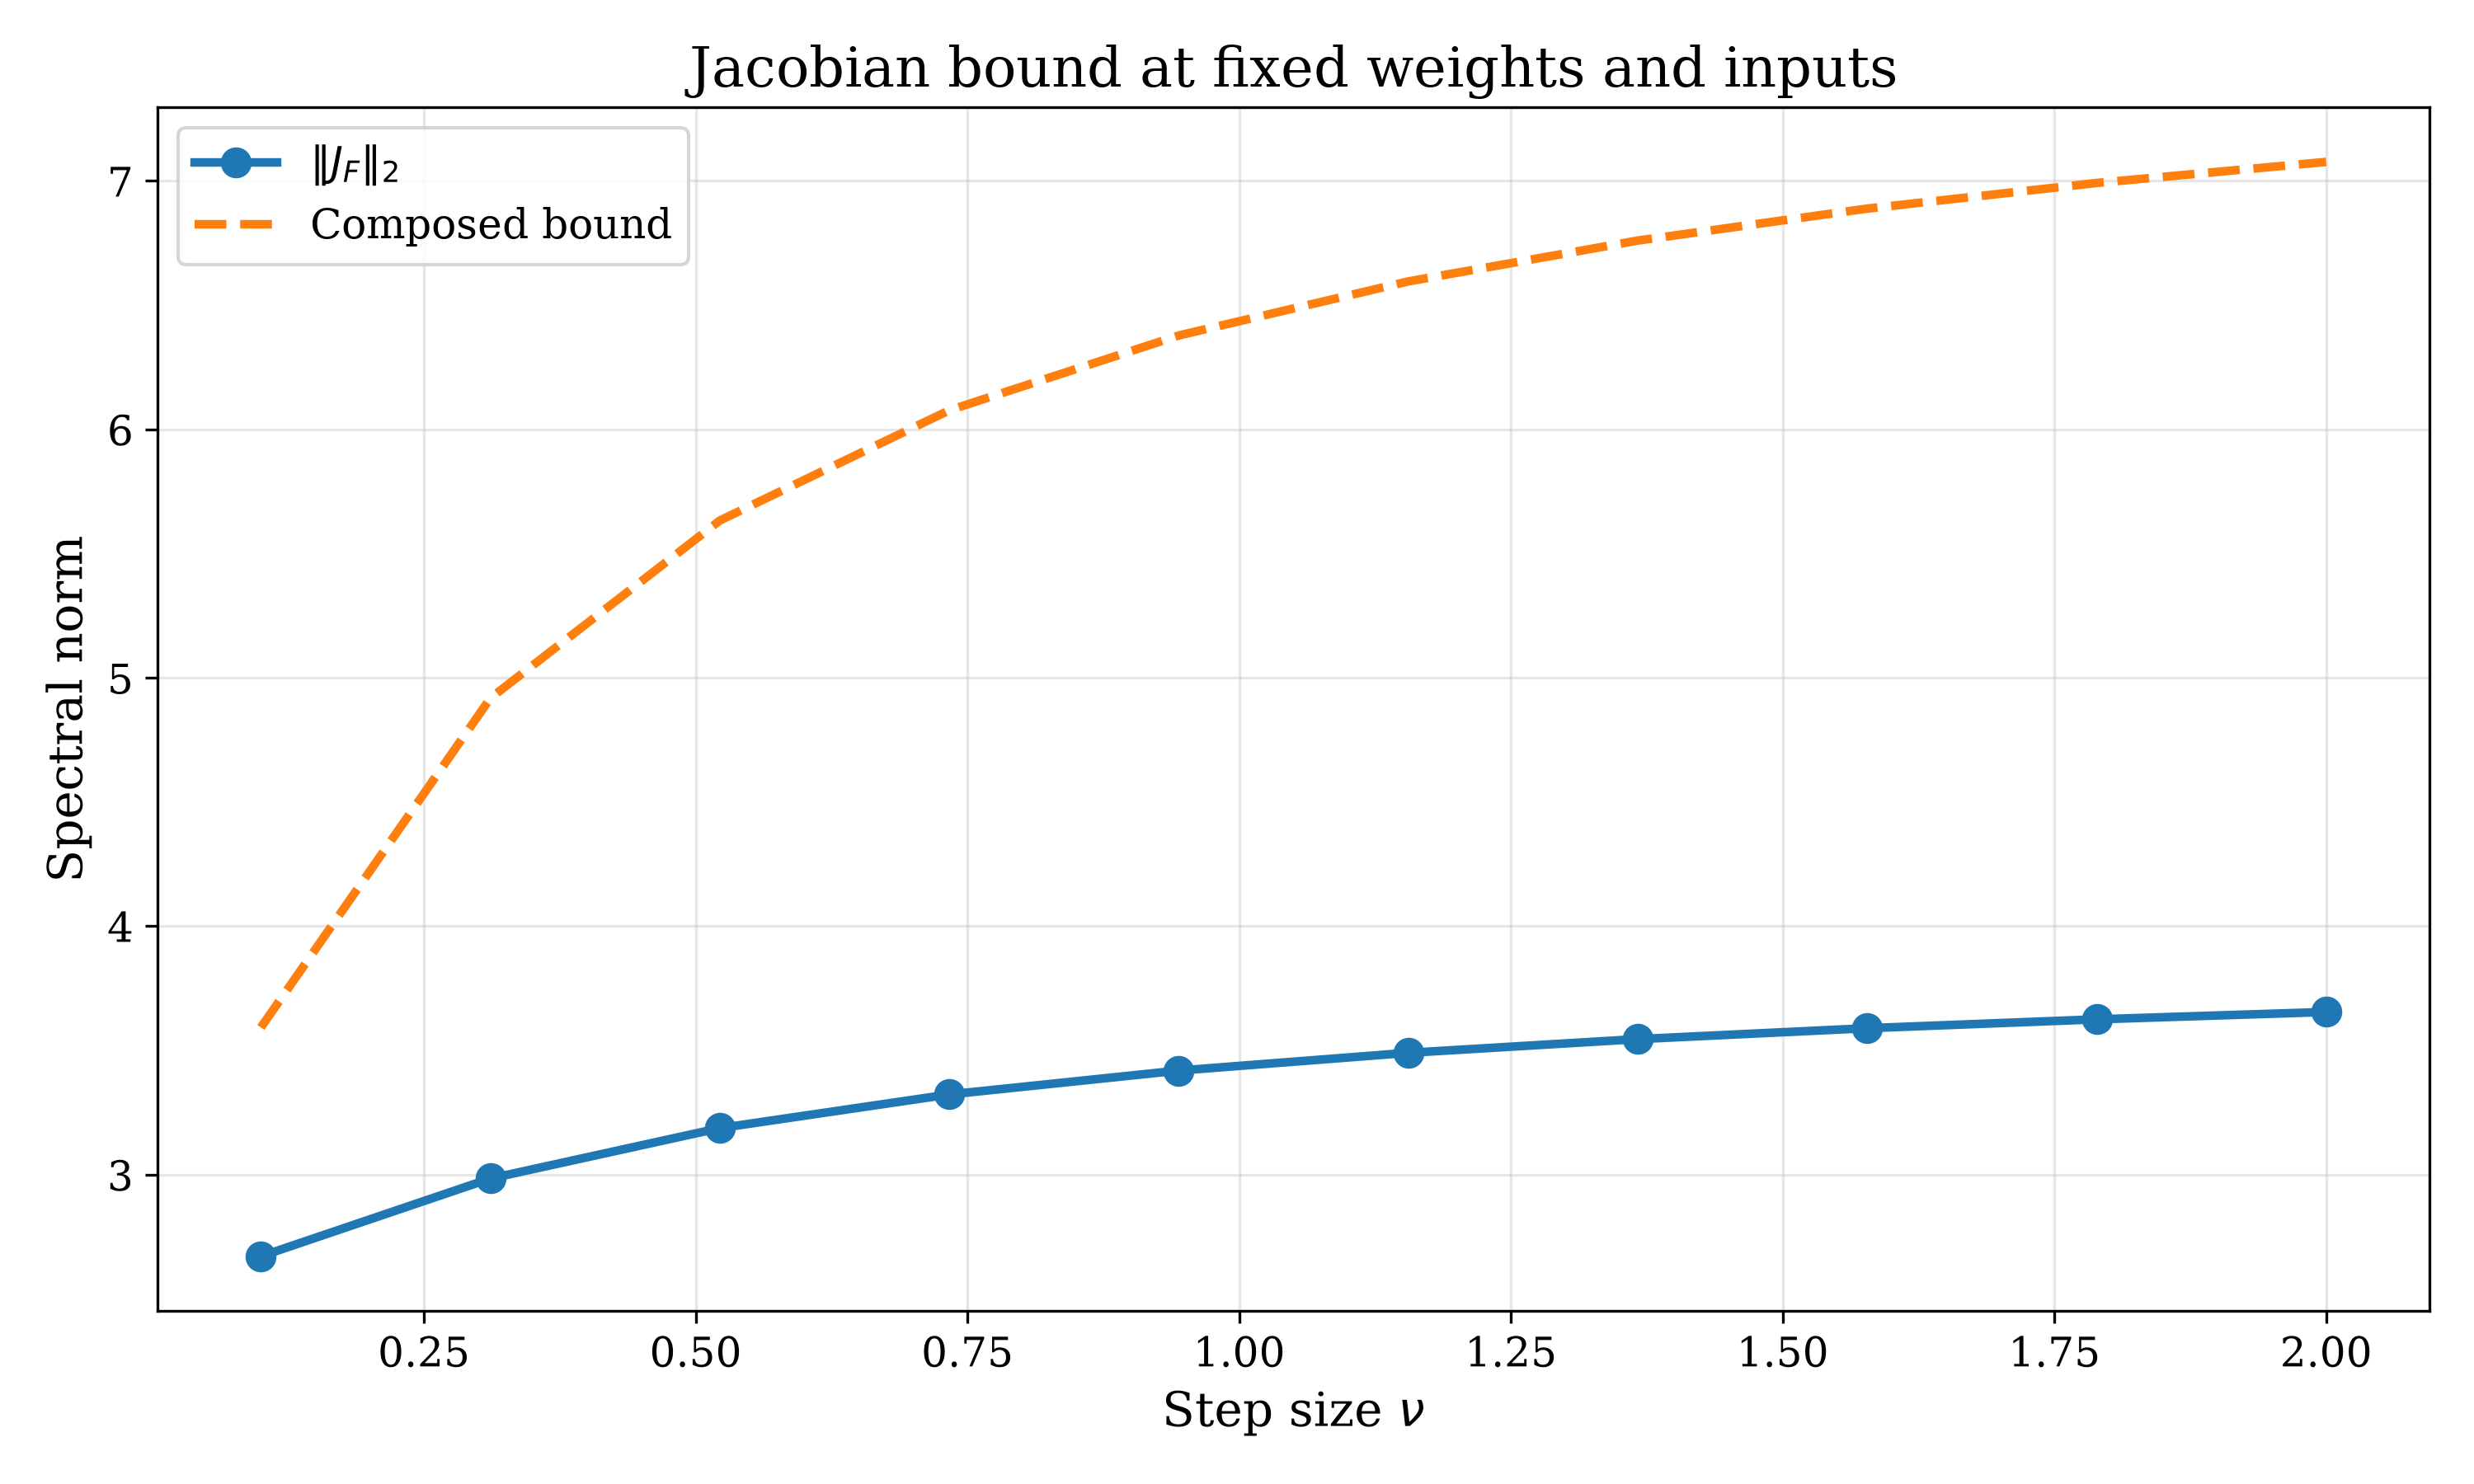
\includegraphics[width=0.85\linewidth]{fig1_bounds_validation.png}
\caption{One-step Jacobian norm and the composed bound for a fixed model,
state, and context. Component norms are computed at the same states used by
the recurrent update.}
\label{fig:bound}
\end{figure}
The measured component norms are $M=0.9607$ and $L=0.5486$. The inequality
holds at all ten sampled step sizes. The one-step norm increases from $2.6713$
at $\nu=0.1$ to $3.6547$ at $\nu=2.0$; the corresponding bounds are $3.5924$
and $7.0763$. These values illustrate a conservative bound and do not certify
contraction, since the measured norms exceed one.

\subsection{Large-step behavior}
We use the same dimensions and Gaussian distributions, with seeds 0 through 9.
Each seed specifies a model, state, and context that remain fixed across twenty
logarithmically spaced values of $\nu$ from $10^{-1}$ to $10^5$. Means and
standard deviations are taken across these ten independent repetitions, rather
than across inputs to a single model newly sampled at each step size. This
protocol follows the fixed-parameter scope of Theorem~\ref{thm:asymptotic}.
We also compute the Jacobian of the limiting map
\begin{equation}\label{eq:limitmap}
(G_\infty(Y))_i=\sqrt D\,\diag(\gamma_U)
\frac{\Delta(Y)_i}{\norm{\Delta(Y)_i}_2}.
\end{equation}
Here tokens are written as column vectors. The positive lower bound on the
update norms makes this map differentiable in a neighborhood of the sampled
state. The outer stabilizer vanishes in the limit because it is divided by
$\nu^2$; both inner stabilizers remain part of $\TB$. The reference line in
Figure~\ref{fig:asymptotic} is the mean of
$\norm{D_YG_\infty(Y)}_2$ across seeds, computed separately from the finite-step
curves. It is not the norm of a mean Jacobian or the last sampled ordinate.
\begin{figure}[htbp]
\centering
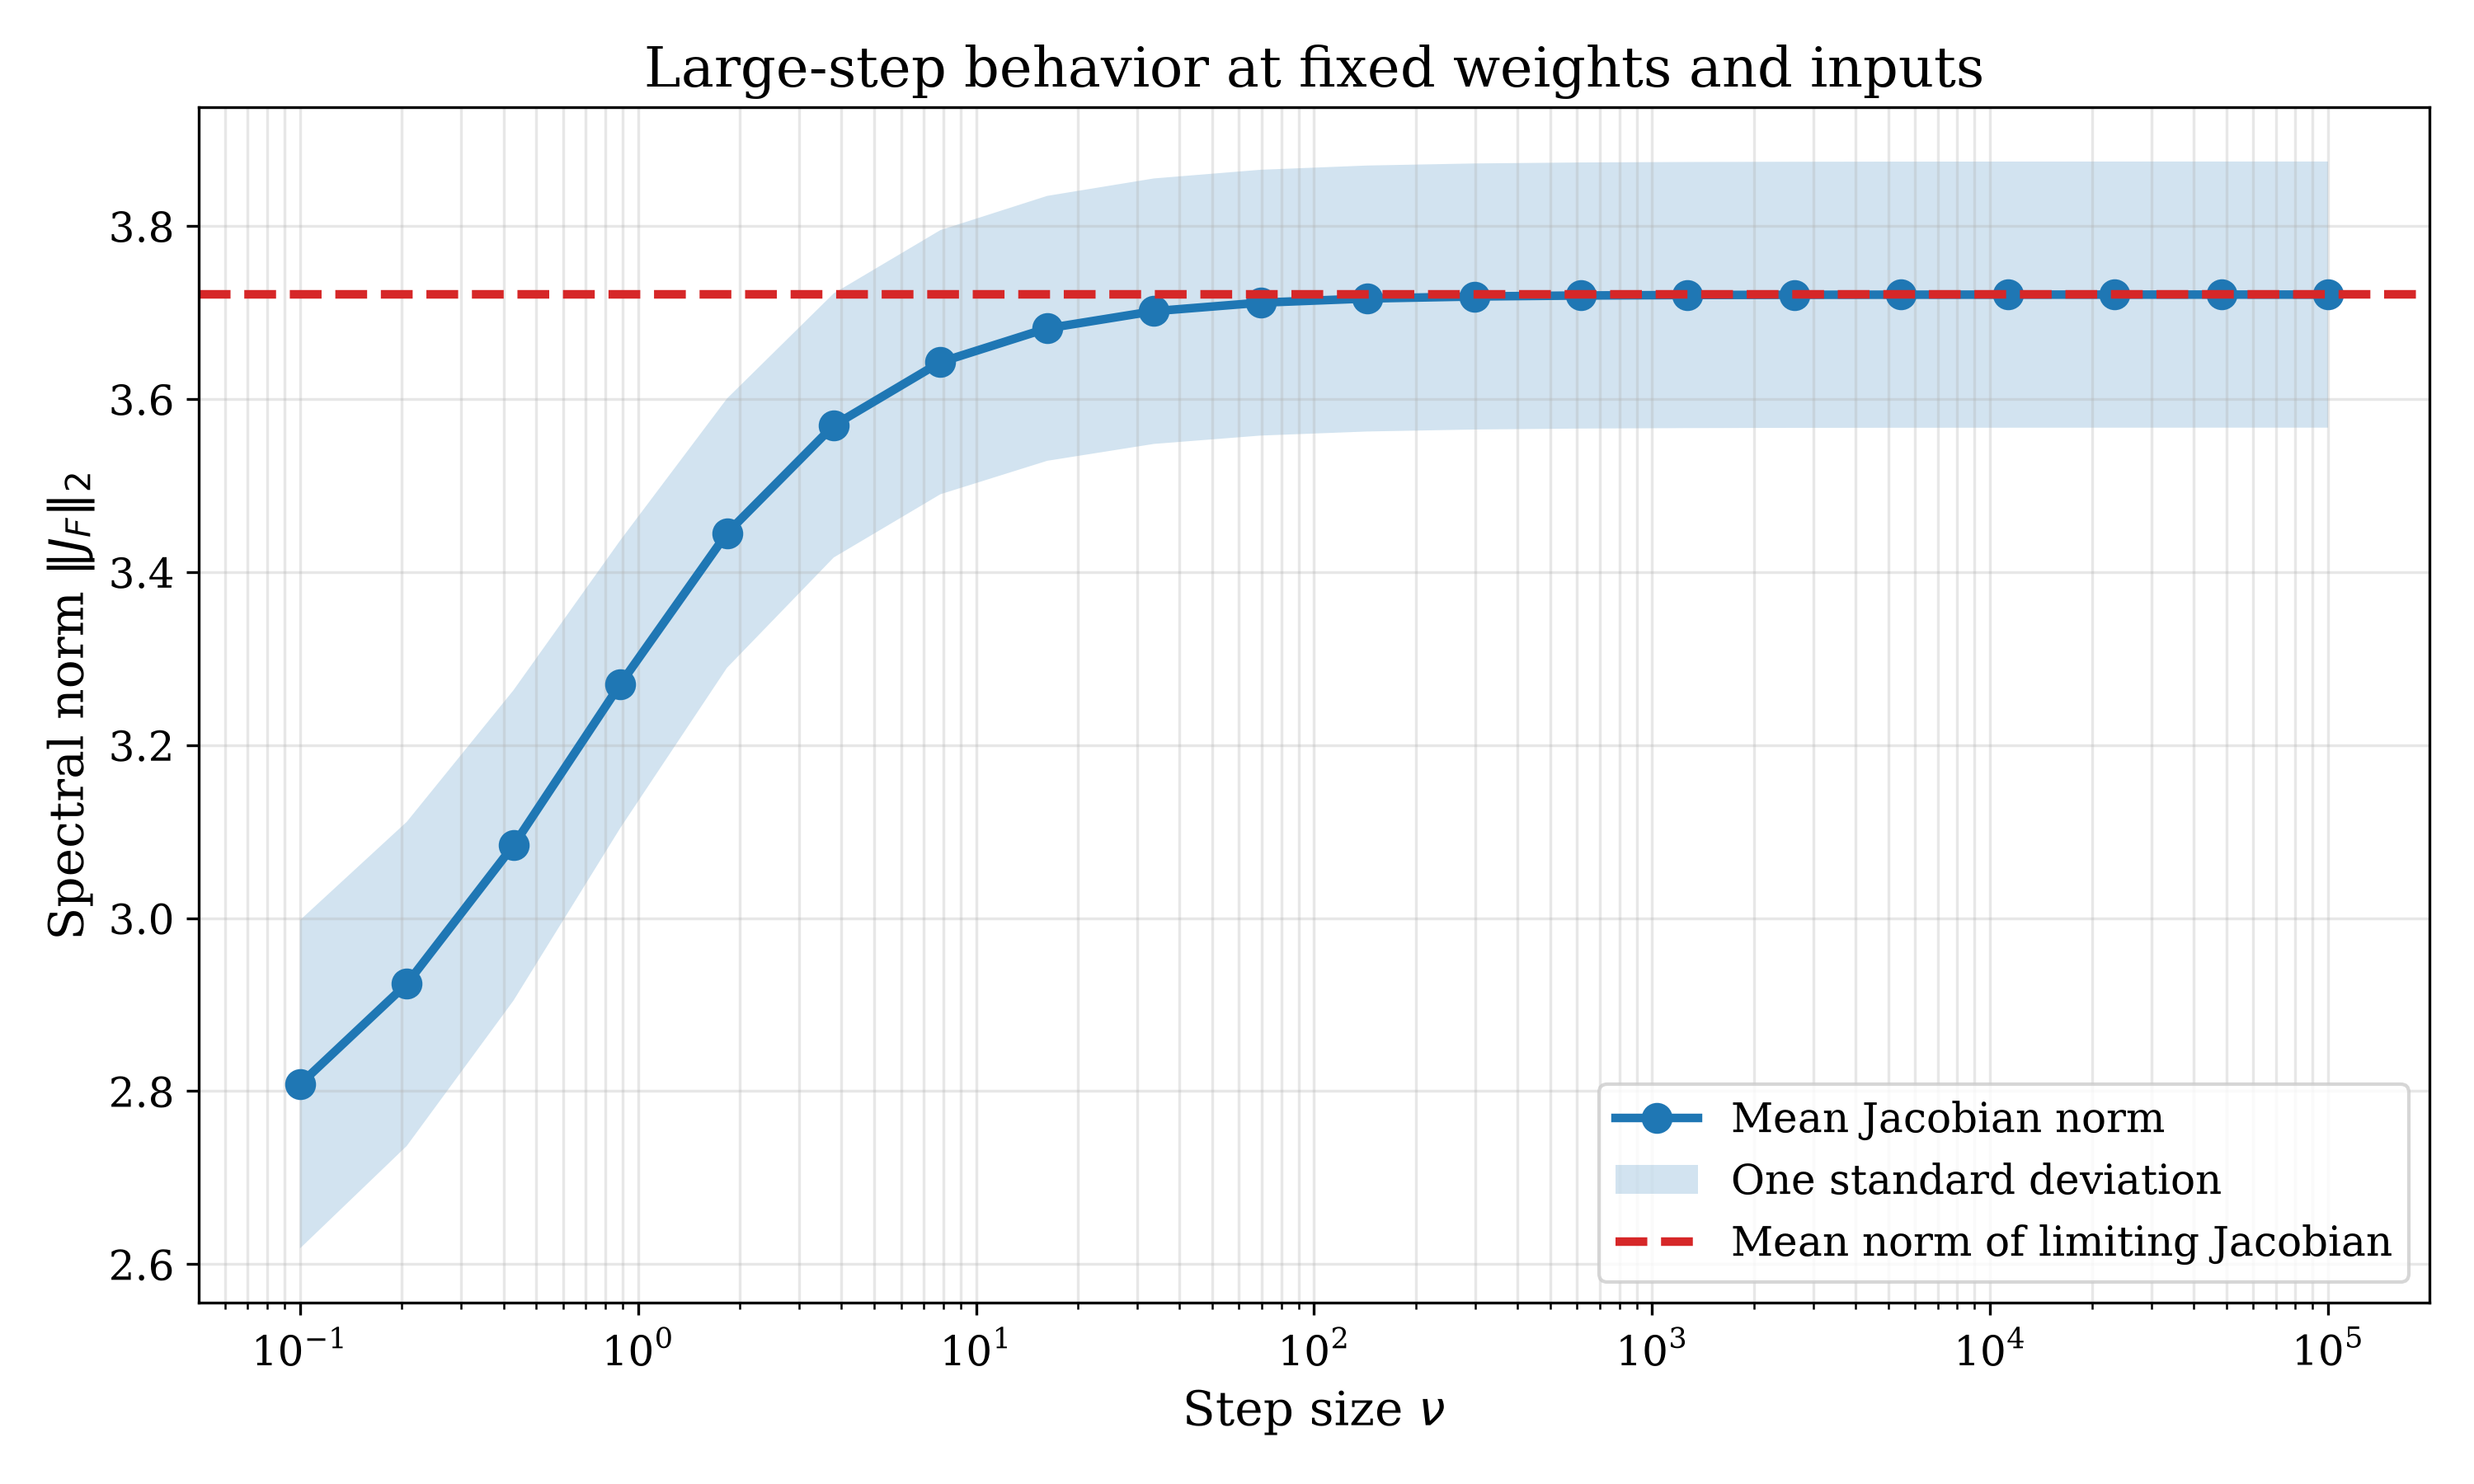
\includegraphics[width=0.85\linewidth]{fig2_asymptotic.png}
\caption{Dependence of the one-step Jacobian norm on step coefficient.
The horizontal axis is logarithmic. The curve is the mean and the band is
one population standard deviation across ten seeds; within each seed only
$\nu$ changes. The dashed reference is the mean norm of the limiting Jacobian.}
\label{fig:asymptotic}
\end{figure}
The mean norm is $2.8079$ at $\nu=0.1$ and $3.720649$ at $\nu=10^5$,
compared with a mean limiting norm of $3.720655$. At the largest step, the
standard deviation across seeds is $0.1538$, and the largest per-seed absolute
difference from the corresponding limiting norm is $7.94\times10^{-6}$.
The smallest update-row norm across the ten runs is $5.4294$, so all sampled
states satisfy the non-degeneracy condition. The finite-step curves are
consistent with the large-step limit; their plateau above one does not imply
contraction.

\subsection{Successive-state differences}
For the trajectory experiment we use $S=32$, $D=64$, $H=4$, and
$D_{\rm ff}=128$. Starting from $Y^{(0)}$, we hold $C=0.1Y^{(0)}$ fixed and
record
\begin{equation}
d_t=\norm{Y^{(t+1)}-Y^{(t)}}_F
\end{equation}
over 1000 steps for $\nu\in\{0.1,0.5,1.0\}$. Inputs are Gaussian sequences
or CIFAR-10 test images~\cite{krizhevsky2009cifar} mapped to sequences using a
random linear projection. The projection and the recurrent block are untrained.
We use seeds 0 through 4, with five Gaussian samples and the five fixed CIFAR-10
test images at indices 0 through 4 for each seed, giving 25 trajectories per
dataset and step size. Each image is scaled to $[-1,1]$, divided by its own
sample standard deviation, reshaped into 32 rows of 96 values, and projected
to dimension 64. For each seed, the same block weights are used for both
datasets and all step sizes. Model weights, Gaussian inputs, and projection
weights use separate random-number streams.

We report the median residual and the observed minimum-to-maximum range.
The finite-run criterion is $d_t\leq10^{-4}$ throughout the final 20 steps;
passing it is not a claim of asymptotic convergence. The trajectories use
float32, so late residuals also depend on numerical precision.
\begin{figure}[htbp]
\centering
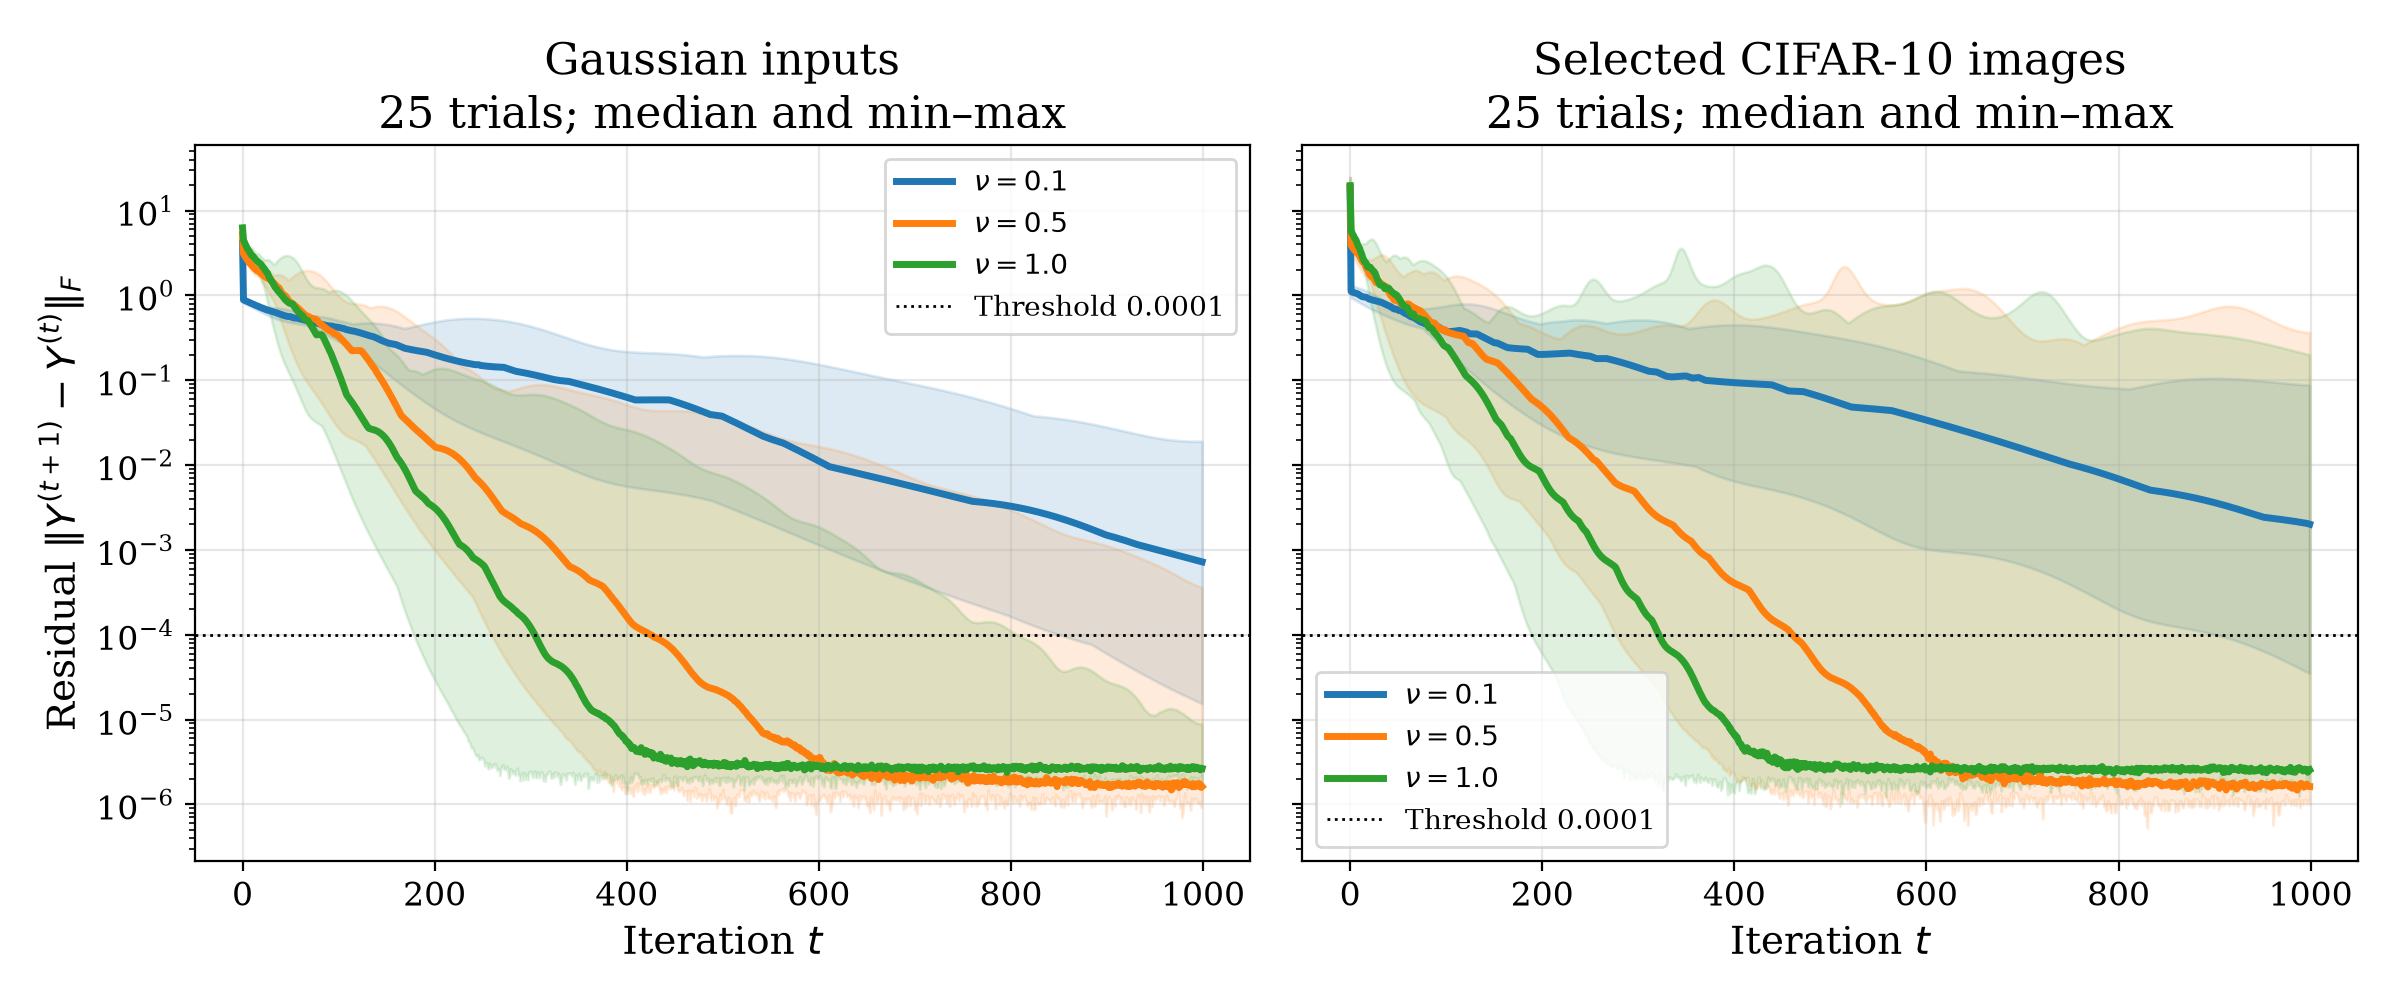
\includegraphics[width=\linewidth]{fig3_contraction.png}
\caption{Successive-state differences on Gaussian inputs and projected
CIFAR-10 images. Lines show medians across 25 trajectories; shaded bands span
the observed minimum and maximum, not confidence intervals. The dotted line
marks the $10^{-4}$ residual threshold.}
\label{fig:dynamics}
\end{figure}
Table~\ref{tab:residuals} gives the number of trajectories meeting the residual
criterion. Some sampled trajectories have not met the threshold after 1000
steps. This does not show that they fail to converge as $t\to\infty$.
For this sample and iteration budget, larger $\nu$ increases the fraction
meeting the criterion; this is an observation about the tested conditions,
not a general monotonicity result.

\begin{table}[htbp]
\centering
\caption{Trajectories with $d_t\leq10^{-4}$ throughout the final 20 of
1000 steps. Each entry is a count out of 25 trajectories.}
\label{tab:residuals}
\begin{tabular}{lccc}
\toprule
Input & $\nu=0.1$ & $\nu=0.5$ & $\nu=1.0$\\
\midrule
Gaussian & 6/25 & 23/25 & 25/25\\
CIFAR-10 & 6/25 & 20/25 & 22/25\\
\bottomrule
\end{tabular}
\end{table}

Zero residuals are displayed at $10^{-12}$ on the logarithmic plot; the saved
arrays retain their original values. A decrease in $d_t$ over a finite run is
evidence about those trajectories only.
Even the asymptotic condition $d_t\to0$ alone is not a general proof that a
sequence converges. The experiment therefore supplies no global convergence
guarantee.

\section{Conclusion}
The chain rule extends the recurrent self-attention Jacobian bound to a block
with a feed-forward network and two inner RMSNorm layers. The estimate uses
separate normalization scales and the smallest RMS denominator at each layer.
For fixed inputs and parameters, a nonzero per-token update makes the outer
denominator grow with $\nu$, compensating for the explicit step multiplier.
This establishes boundedness of the one-step Jacobian in the large-step limit.
Contraction, stability over many steps, and behavior of trained networks require
additional conditions or measurements.

\appendix
\section{Proofs}
\subsection{Derivative of RMSNorm}
\begin{lemma}\label{lem:rms}
For $R(y)=\diag(\gamma)y/\rho(y)$ with
$\rho(y)=\sqrt{\norm{y}_2^2/D+\epsilon}$ and $\epsilon>0$,
\begin{equation}\label{eq:rmsjac}
J_R(y)=\frac{\diag(\gamma)}{\rho(y)}
\left(I-\frac{yy^\top}{D\rho(y)^2}\right),\qquad
\norm{J_R(y)}_2\leq\frac{\norm{\gamma}_\infty}{\rho(y)}.
\end{equation}
\end{lemma}
\begin{proof}
Differentiation gives $\nabla\rho(y)=y/(D\rho(y))$, and the product rule
gives Eq.~\eqref{eq:rmsjac}. The matrix in parentheses has eigenvalue one in
directions orthogonal to $y$, and eigenvalue $\epsilon/\rho(y)^2$ in the
direction of $y$. Both lie in $[0,1]$. At $y=0$ the matrix is the identity.
Submultiplicativity yields the stated inequality. Row-wise normalization has
a block-diagonal Jacobian, so its norm is bounded by the maximum token bound.
\end{proof}
For $\epsilon=0$ and nonzero input, the matrix in parentheses is the tangent
projector. This recovers Lemma A.3 of~\cite{tomihari2025recurrent}, after
accounting for the $\sqrt D$ scale convention. At the outer layer the derivative
is evaluated at $U_\nu$, not at the incoming state $Y$; with positive $\epsilon$
the matrix is no longer an exact projector.

\subsection{Proof of Theorem~\ref{thm:bound}}\label{app:bound}
The chain rule gives
\begin{align}
J_{\TB}(Y)
&=J_{R_2}(Z_2)(I+J_{\FFN}(Y'))J_{R_1}(Z_1)(I+J_{\MSA}(Y)),\\
J_{F_\nu}(Y)&=J_{R_U}(U_\nu)(I+\nu J_{\TB}(Y)).
\end{align}
Lemma~\ref{lem:rms} and the block-diagonal norm identity imply
\begin{equation}
\norm{J_{\TB}(Y)}_2
\leq\frac{g_2}{r_2}(1+L)\frac{g_1}{r_1}(1+M)=K.
\end{equation}
Substitution into
$\norm{J_{F_\nu}(Y)}_2\leq(g_U/r_U)(1+\nu\norm{J_{\TB}(Y)}_2)$
proves Eq.~\eqref{eq:bound}.\qed

\subsection{Proof of Theorem~\ref{thm:asymptotic}}\label{app:asymptotic}
For every token, the reverse triangle inequality gives
\begin{equation}
\norm{(U_\nu)_{[i,:]}}_2
\geq\nu\norm{\Delta(Y)_{[i,:]}}_2-\norm{Y_{[i,:]}}_2
\geq\nu\delta-B.
\end{equation}
For $\nu\geq2B/\delta$ this is at least $\nu\delta/2$. Consequently
\begin{equation}
r_U=\min_i\sqrt{\norm{(U_\nu)_{[i,:]}}_2^2/D+\epsilon_U}
\geq\frac{\nu\delta}{2\sqrt D}.
\end{equation}
The inner states and $K$ are independent of $\nu$ because $Y$, $C$, and all
parameters are fixed. Theorem~\ref{thm:bound} now yields
\begin{equation}
\norm{J_{F_\nu}(Y)}_2
\leq\frac{2\sqrt D\,g_U}{\nu\delta}(1+\nu K),
\end{equation}
which is Eq.~\eqref{eq:asymptotic}. This argument does not assume that $Y$ was
produced by a preceding normalization.\qed

\bibliographystyle{plain}
\bibliography{references}
\end{document}
